\documentclass[12pt]{article}
\setcounter{secnumdepth}{3}

\usepackage[margin=1in]{geometry} 
\usepackage{amsmath,amsthm,amssymb,color}
\usepackage{graphicx}
\usepackage{mathtools}
\usepackage[section]{placeins}
\usepackage{listings}
\usepackage{mathdots}
\usepackage{centernot}
\usepackage{algorithm}
\usepackage[noend]{algpseudocode}
\usepackage{csquotes}
\usepackage[table,xcdraw]{xcolor}
\usepackage{booktabs}
\usepackage{cite}
\usepackage{enumerate}
\usepackage{tikz}
\usetikzlibrary{calc}
\usepackage{bbm}
\usetikzlibrary{arrows, shapes}
\usetikzlibrary{patterns}
\usepackage{natbib}
\usepackage{relsize}
\usepackage{booktabs}
\usetikzlibrary{decorations.pathreplacing}
\allowdisplaybreaks


\usepackage{hyperref}
\hypersetup{
    colorlinks,
    citecolor=black,
    filecolor=black,
    linkcolor=black,
    urlcolor=black
}

\DeclarePairedDelimiter\ceil{\lceil}{\rceil}
\DeclarePairedDelimiter\floor{\lfloor}{\rfloor}
 
\newcommand\scalemath[2]{\scalebox{#1}{\mbox{\ensuremath{\displaystyle #2}}}}

\newcommand{\N}{\mathcal{N}}
\newcommand{\Z}{\mathbb{Z}}
\newcommand\independent{\protect\mathpalette{\protect\independenT}{\perp}}
\def\independenT#1#2{\mathrel{\rlap{$#1#2$}\mkern2mu{#1#2}}}

\theoremstyle{plain}
\newtheorem{thm}{Theorem}%[section]
\theoremstyle{plain}
\newtheorem{lem}{Lemma}%[section]
\theoremstyle{plain}
\newtheorem{prop}{Proposition}%[section]
\theoremstyle{plain}
\newtheorem{cor}{Corollary}%[thm]
\theoremstyle{plain}
\newtheorem{defin}{Definition}%[section]
\theoremstyle{remark}
\newtheorem{rem}{Remark}%[section]
\theoremstyle{plain}
\newtheorem{exe}{Exercise}%[section]
\theoremstyle{plain}
\newtheorem{exa}{Example}%[section]
\theoremstyle{plain}
\newtheorem{fact}{Fact}%[section]
\theoremstyle{discussion}
\newtheorem{discussion}{Discussion}%[section]
\theoremstyle{plain}
\newtheorem{conj}{Conjecture}%[section]

\newcommand{\wtil}{\widetilde}
\newcommand{\inte}{\mathrm{int}}
\newcommand{\iid}{\stackrel{\text{iid}}{\sim}}
\newcommand{\eqe}{\stackrel{\cdot}{=}}
\newcommand{\ft}{\mathcal{F}}
\newcommand{\mm}{S}
\newcommand{\spa}{\mathrm{Spa}}
\newcommand{\sm}{\widehat{\mathrm{M}}}
\newcommand{\dou}{\mathrm{Doub}}
\newcommand{\cir}{\mathrm{Circ}}
\newcommand{\supp}{\mathrm{supp}}
\newcommand{\M}{\mathcal{M}}
\newcommand{\F}{\mathbb{F}}
\newcommand{\mR}{\mathbb{R}}
\newcommand{\mN}{\mathbb{N}}
\newcommand{\mZ}{\mathbb{Z}}
\newcommand{\mC}{\mathbb{C}}
\newcommand{\mQ}{\mathbb{Q}}
\newcommand{\mF}{\mathbb{F}}
\newcommand{\iim}{\mathrm{Im}\:}
\newcommand{\re}{\mathrm{Re}\:}
\newcommand{\tr}{\mathrm{tr}}
\newcommand{\Corr}{\mathrm{corr}}
\newcommand{\Cov}{\mathrm{cov}}
\newcommand{\pp}{\mathbb{P}}
\newcommand{\E}{\mathbb{E}}
\DeclareMathOperator{\Var}{Var}
\newcommand{\e}{\varepsilon}
\newcommand{\ent}{h}
\newcommand{\info}{I}
\newcommand{\rank}{\mathrm{rank}}
\newcommand{\nullity}{\mathrm{nullity}}
\DeclareMathOperator{\diag}{diag}
\newcommand{\cS}{\mathcal{S}}
\newcommand{\cT}{\mathcal{T}}
\newcommand{\X}{\mathcal{X}}
\newcommand{\Y}{\mathcal{Y}}
\newcommand{\I}{\mathcal{I}}
\newcommand{\D}{\mathcal{D}}
\newcommand{\C}{\mathcal{C}}
\newcommand{\B}{\mathcal{B}}
\newcommand{\Po}{\mathcal{P}}
\newcommand{\Tr}{\text{Trace}}
\newcommand\mapsfrom{\mathrel{\reflectbox{\ensuremath{\mapsto}}}}

\definecolor{amethyst}{rgb}{0.6,0.4,0.8}


\begin{document}

\begin{figure}
\label{fig:naive_mandelian}
\begin{center}
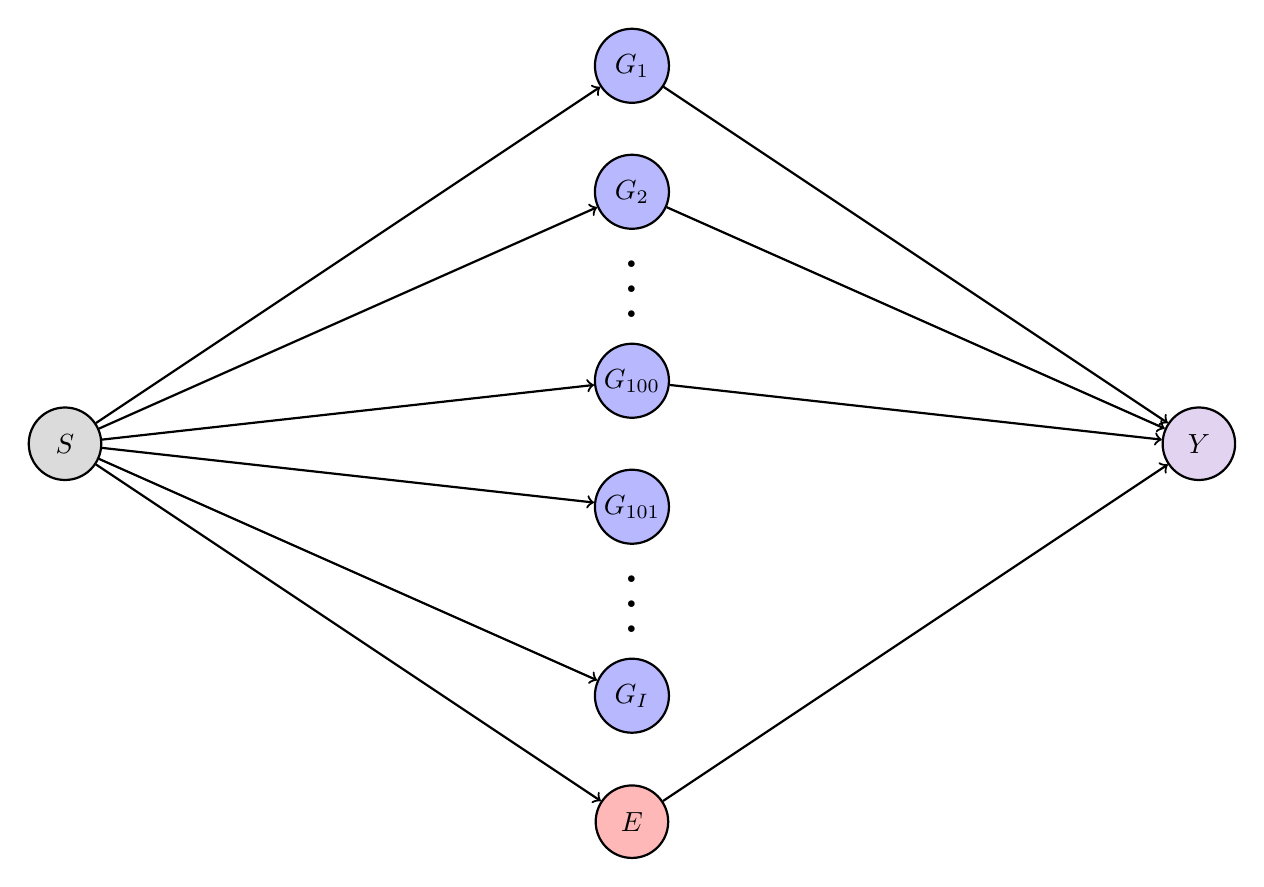
\begin{tikzpicture}[scale = 0.8, rotate=90]
\tikzstyle{vertex_y}=[circle, thick, fill=amethyst!28, draw=black, text width = 8mm, align = center, inner sep=1pt]
\tikzstyle{vertex_s}=[circle, thick, fill=gray!28, draw=black, text width = 8mm, align = center, inner sep=1pt]
\tikzstyle{vertex_e}=[circle, thick, fill=red!28, draw=black, text width = 8mm, align = center, inner sep = 1pt]
\tikzstyle{vertex_x}=[circle, thick, fill=blue!28, draw=black, text width = 8mm, align = center, inner sep = 1pt]

\path (0, 18) node[vertex_s](S) {$S$}
	  (-6, 9) node[vertex_e](E1) {$E$}
	  (6, 9) node[vertex_x](G1) {$G_1$}
	  (4, 9) node[vertex_x](G2) {$G_2$}
	  (1, 9) node[vertex_x](G10) {$G_{100}$}
	  (-1, 9) node[vertex_x](G11) {$G_{101}$}
	  (-4, 9) node[vertex_x](Gm) {$G_I$}
	  (0,0) node[vertex_y](Y) {$Y$};

\draw[->, line width = .8] (S) -- (G1);
\draw[->, line width = .8] (S) -- (G2);
\draw[->, line width = .8] (S) -- (G10);
\draw[->, line width = .8] (S) -- (G11);
\draw[->, line width = .8] (S) -- (Gm);
\draw[->, line width = .8] (S) -- (E1);
\draw[->, line width = .8] (E1) -- (Y);
\draw[->, line width = .8] (G1) -- (Y);
\draw[->, line width = .8] (G2) -- (Y);
\draw[->, line width = .8] (G10) -- (Y);
\path (G11) + (-0.1,0) -- (Gm) node [font=\Huge, midway, sloped] {$\vdots$};
\path (G2) + (-0.1,0) -- (G10) node [font=\Huge, midway, sloped] {$\vdots$};

\end{tikzpicture}
\end{center}
\end{figure}

\end{document}